
\section*{Visualización de Resultados del Modelo de Regresión Logística}

\subsection*{Curva ROC}
La curva ROC muestra la sensibilidad frente a 1 - especificidad, permitiendo evaluar la capacidad del modelo para discriminar entre los casos con y sin cáncer. Un área bajo la curva (AUC) cercana a 1 indica excelente discriminación.

\begin{figure}[h!]
\centering
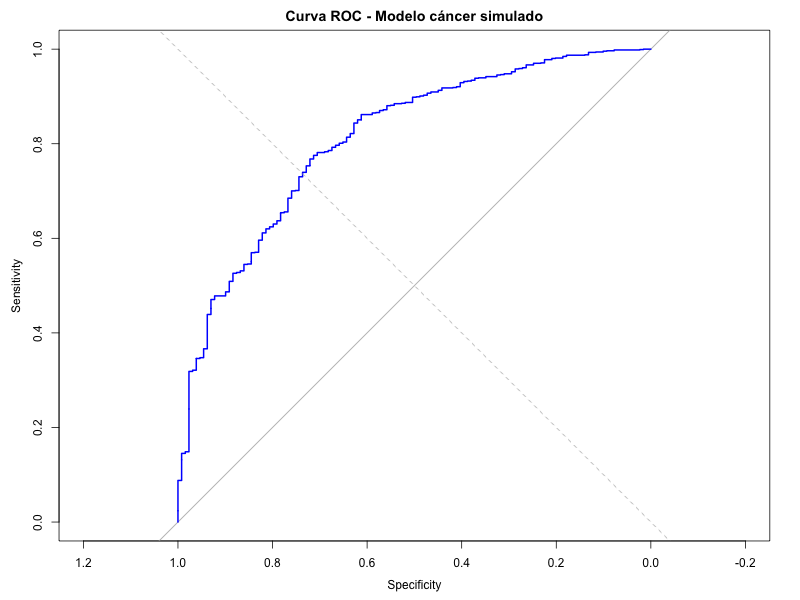
\includegraphics[width=0.75\textwidth]{curva_roc.png}
\caption{Curva ROC del modelo logístico ajustado}
\end{figure}

\subsection*{Histograma de Probabilidades Predichas}
Este histograma muestra la distribución de las probabilidades predichas por el modelo. Permite visualizar la concentración de predicciones cercanas a los extremos 0 o 1.

\begin{figure}[h!]
\centering
\includegraphics[width=0.75\textwidth]{hist_probabilidades.png}
\caption{Distribución de las probabilidades predichas por el modelo}
\end{figure}

\subsection*{Gráfico de Efectos (Odds Ratios)}
El siguiente gráfico presenta los efectos de cada predictor en forma de Odds Ratio junto con sus intervalos de confianza al 95\%. Las líneas discontinuas indican el valor de referencia (OR = 1).

\begin{figure}[h!]
\centering
\includegraphics[width=0.75\textwidth]{efectos_logisticos.png}
\caption{Odds Ratios con intervalos de confianza al 95\%}
\end{figure}
